\phantomsection
\section{Entities and relations in UML.}
\begin{flushleft}
\setlength{\parindent}{2ex}
\par
The \textbf{Unified Modeling Language} is a widely accepted language used by analysts and software developers that is an excellent fit for the graphic representation of \textbf{Entity Relationship Diagrams}.
\par 
An \textbf{Entity Relationship Diagram} is a representation of data within a domain. It consists of entities as well as relationships between entities.
\par 
The are four elements of Entities:
\begin{enumerate}
		\item[•]Structural
    	\item[•]Behavioral 
    	\item[•]Grouping
    	\item[•]Annotational
\end{enumerate}
\end{flushleft}
\textbf{Structural} Entities define the static part of the model. They represent the physical and conceptual elements.
\begin{enumerate}
\item \textbf{Class} - defines a set of objects having similar attributes and methods.
\begin{figure}[h]
\centering
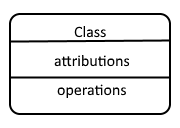
\includegraphics[keepaspectratio=true,scale=1]{class}
\caption{Class}
\end{figure}
\par
\noindent
Attributions of a class can be:
\begin{enumerate}
		\item[•] public: +
    	\item[•] private: - 
    	\item[•] protected: \#
\end{enumerate} \par
\item \textbf{Interface} - defines a set of operations, which specify the responsibility of a class.
\begin{figure}[h]
\centering
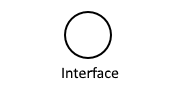
\includegraphics[keepaspectratio=true,scale=1]{interface}
\caption{Interface}
\end{figure}\newpage
\item \textbf{Collaboration} - defines an interaction between elements.
\begin{figure}[h]
\centering
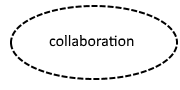
\includegraphics[keepaspectratio=true,scale=1]{colaboration}
\caption{Collaboration}
\end{figure}
\item \textbf{Use case} - represents a set of actions performed by a system for a specific goal.
\begin{figure}[h]
\centering
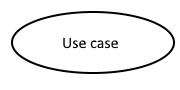
\includegraphics[keepaspectratio=true,scale=1]{usecase}
\caption{Use Case}
\end{figure}
\item \textbf{Active class} - are the classes who's objects are already used in processes or threads. Graphically it is the same class
\item \textbf{Component} describes the physical part of a system.
\begin{figure}[h]
\centering
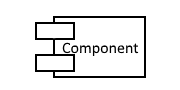
\includegraphics[keepaspectratio=true,scale=1]{component}
\caption{Component}
\end{figure}
\item \textbf{Node} - can be defined as a physical element that exists at run time.
\begin{figure}[h!]
\centering
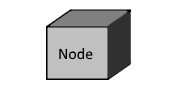
\includegraphics[keepaspectratio=true,scale=1]{node}
\caption{Node}
\end{figure}
\end{enumerate}
While their operations/methods distinctive to their cases.
%next after structure-----------------------------------------------------------------------------------
\newpage
\par
\noindent
\textbf{Behavioral} entities are dynamic parts of the UML model.
\begin{enumerate}
\item \textbf{Interaction} - is defined as a behavior that consists of a group of messages exchanged among elements to accomplish a specific task.
\begin{figure}[h!]
\centering
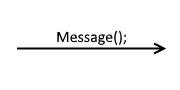
\includegraphics[keepaspectratio=true,scale=1]{interaction}
\caption{Message}
\end{figure}
\item \textbf{State machine(Automata)} - used when the state of an object in its life cycle is important. It defines the sequence of states an object goes through in response to events. Events are external factors responsible for state change.
\begin{figure}[h!]
\centering
\includegraphics[keepaspectratio=true,scale=1]{state}
\caption{States}
\end{figure}
\end{enumerate}
\par
\noindent
\textbf{Grouping} - defined as a mechanism to group elements of a UML model together
\begin{enumerate}
\item \textbf{Package} - the only one grouping entity available for gathering structural and behavioral entities.
\begin{figure}[h!]
\centering
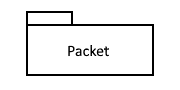
\includegraphics[keepaspectratio=true,scale=1]{packet}
\caption{Package} 
\end{figure}
\end{enumerate}
\par
\noindent
\textbf{Annotational} Annotational entities can be defined as a mechanism to capture remarks, descriptions, and comments of UML model elements.
\begin{figure}[h!]
\centering
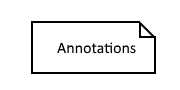
\includegraphics[keepaspectratio=true,scale=1]{annotations}
\caption{Annotation} 
\end{figure}
\newpage
\section{Project description.}
The \textbf{Tracking System} is a multipurpose tracking system which can help in tracking the data on a computer.This can be used in various ways like History based tracking in case the user had an important work that he would want to remember each step done for offline working routine, or in case of an organization to supervise the work of its employees. When the soft is initialized it opens up in offline mode and has interface methods to extend to an online mode which can add the ID’s of the other users in order to create an Admin Supervisor.The Admin supervisor has control over all the options in whole group. The Interface of the Tracking system contains various additional options in order to be able to create new tracking methods and filter the final data in form of Report for a filtered method.
The filtered method can create or import methods for data filtering. The tracking methods can be chosen in a checkbox form.The default tracking methods will contain Keyboard type tracking,Mouse tracking,Upload/Download data track and a low quality(for fast data transmition) screenshot during a chosen time interval and/or activity.More tracking methods can be further added in the system, in of themselves the tracking methods are mini systems made to work on specific tasks.
\begin{figure}[h!]
\centering
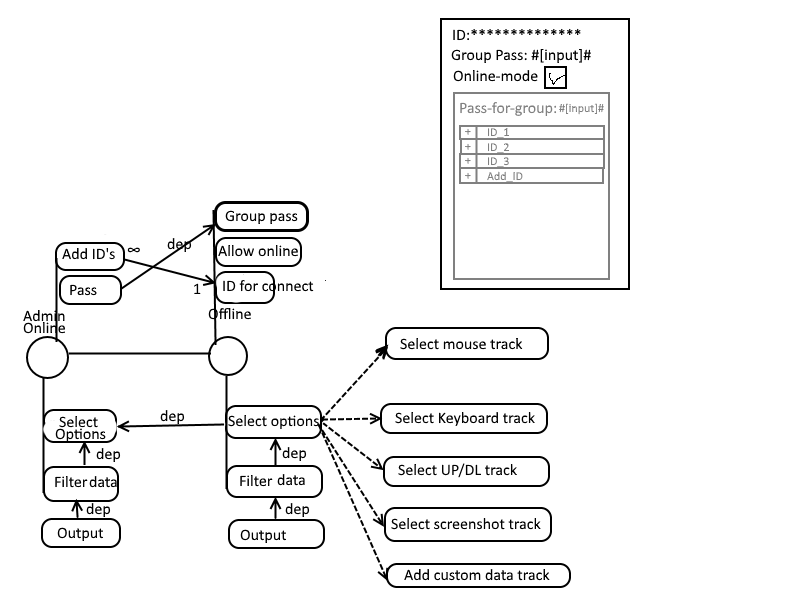
\includegraphics[keepaspectratio=true,scale=0.8]{exampled}
\caption{example} 
\end{figure}
\clearpage
